\section{Bộ dữ liệu ABIDE II}

\subsection{Tải dữ liệu và tổng quan về dữ liệu}
\paragraph{}{Bộ cơ sở dữ liệu \textbf{ABIDE II} \cite{DiMartino2017abideII} được giới thiệu ở NeuroHackademy 2020 bới giáo sư Tal Yarkoni.
Bộ dữ liệu đã được thay đổi một ít để phù hợp với lab này, cụ thể sẽ là phân cụm bệnh nhân có bị ung thư (cancer) hay không (normal).}

\paragraph{}{Dữ liệu được cung cấp trong file \texttt{ABIDE2(updated).csv}, trong đó:}

\begin{itemize}
    \item Số dòng: 1004. Trong đó có 463 bệnh nhân bị ung thư và 541 bệnh
nhân không bị ung thư.
    \item  Số cột: 1444
    \begin{itemize}
    \item \texttt{Unnamed: 0}: Chỉ số dòng (index)
    \item \texttt{Site}: Nơi thu thập dữ liệu (ví dụ: \texttt{ABIDEII-KKI\_1})
    \item \texttt{Subject}: ID của đối tượng nghiên cứu
    \item \texttt{Age}: Tuổi của đối tượng
    \item Các chỉ số còn lại là dữ liệu đặc trưng về não bộ
    \begin{itemize}
        \item Tiền tố \texttt{\texttt{fsArea\_}} (FreeSurfer Area): Diện tích bề mặt của một vùng vỏ não (mm\textsuperscript{2}).
        \item Tiền tố \texttt{\texttt{fsVol\_}} (FreeSurfer Volume): Thể tích của một vùng vỏ não hoặc cấu trúc dưới vỏ não (mm\textsuperscript{3}). 
        \item Tiền tố \texttt{\texttt{fsLGI\_}} (FreeSurfer Local Gyrification Index): Là một thước đo mức độ gấp cuộn của vỏ não tại một vùng cụ thể. Chỉ số này phản ánh mức độ phức tạp của các nếp cuộn não (gyri) và rãnh não (sulci) ở quy mô cục bộ.
        \item Tiền tố \texttt{\texttt{fsCT\_}} (FreeSurfer Cortical Thickness): Độ dày của vỏ não (mm).
 \newline
 \texttt{Chữ cái \texttt{L} và \texttt{R}} trong tên cột: biểu thị bán cầu não trái (\textit{Left}) hoặc phải (\textit{Right}).

   \item \textbf{ROI}: \textit{Region of Interest} – Vùng quan tâm trong nghiên cứu ảnh não.
  
    \end{itemize}
\item \texttt{Group}. Cột này gồm  2 giá trị là: \texttt{Cancer} và \texttt{Normal}.
    \end{itemize}
\end{itemize}

\subsection{Phân tích và dự đoán bệnh nhân}

\paragraph{}{Sau khi dùng chuẩn hóa \textbf{Z-score} và phân tích thành phần chính (\textbf{PCA}) trên bộ dữ liệu ABIDE II, chúng ta thu được:}
\begin{itemize}
    \item \textbf{EVR} (Explained variance ratio) được nắm giữ bởi thành phần chính thứ nhất (PC1) và thành phần chính thứ hai (PC2) lần lượt là \texttt{0.08663063}  và \texttt{0.06472462}.
    \item \textbf{CEVR} (Cumulative explained variance ratio) của PC1 và PC2 là \texttt{0.15135524985487855}.
    \item \textbf{CEVR} của 200 thành phần chính đầu tiên thì đạt gần tới \texttt{0.95}.
\end{itemize}

\begin{figure}[H]
    \centering
    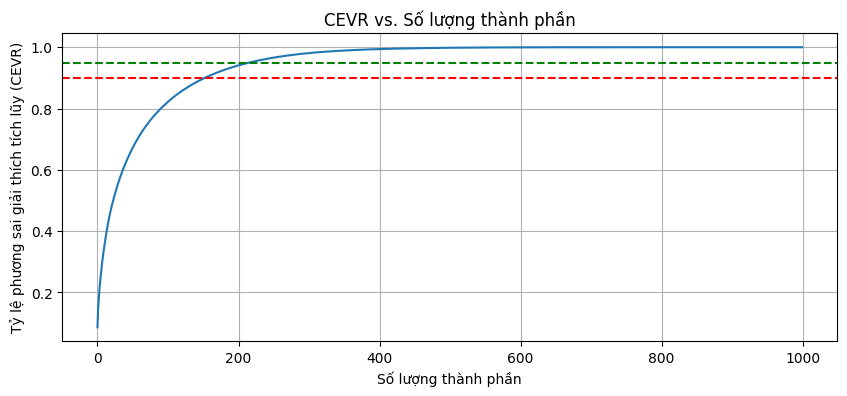
\includegraphics[width=1\linewidth]{img/all_cevr.png}
    \caption{CEVR tương ứng với số lượng thành phần chính}
    \label{fig:all_cevr}
\end{figure}

\paragraph{}{Chúng tôi chọn \texttt{n-components} = 2 cho PCA vì khả năng diễn giải tốt trên mặt phẳng hai chiều và kết quả chấp nhận được với hai thuật toán phân cụm.}

\subsection{Sử dụng thuật toán K-Means}

\paragraph{}{Tiếp theo, ta áp dụng thuật toán k-means với k = 2 và thu được kết quả sau:}

\begin{figure}[H]
    \centering
    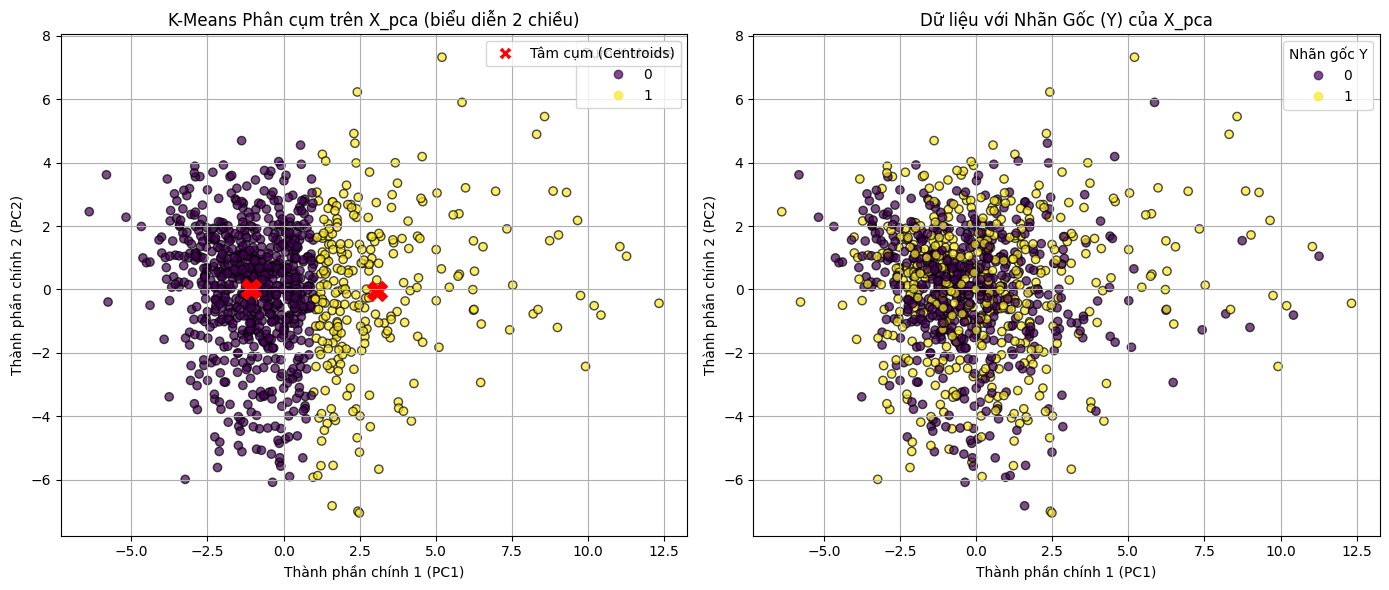
\includegraphics[width=1\linewidth]{img/abideii_plot.png}
    \caption{Kết quả phân cụm bằng KMeans trên bộ dữ liệu ABIDE II}
    \label{fig:abideii_plot}
\end{figure}

\begin{itemize}
    \item Kết quả phân cụm chính xác \textbf{58.1\%} sau khi nối nhãn với cụm phù hợp (bằng thuật toán Hungary). \texttt{Accuracy:} \texttt{0.581}. \texttt{Recall:} \texttt{0.307}. \texttt{Precision:} \texttt{0.587}.  \texttt{F1-score:} \texttt{0.403}. 
    \item Hai cụm dữ liệu thật trên mặt phẳng hai chiều không thể phân biệt rõ được. Tuy nhiên nhãn \texttt{Normal} so với nhãn \texttt{Cancer} có mật độ cao hơn ở trung tâm.
\end{itemize}

\subsection{Sử dụng thuật toán GMM}

\begin{figure}[H]
    \centering
    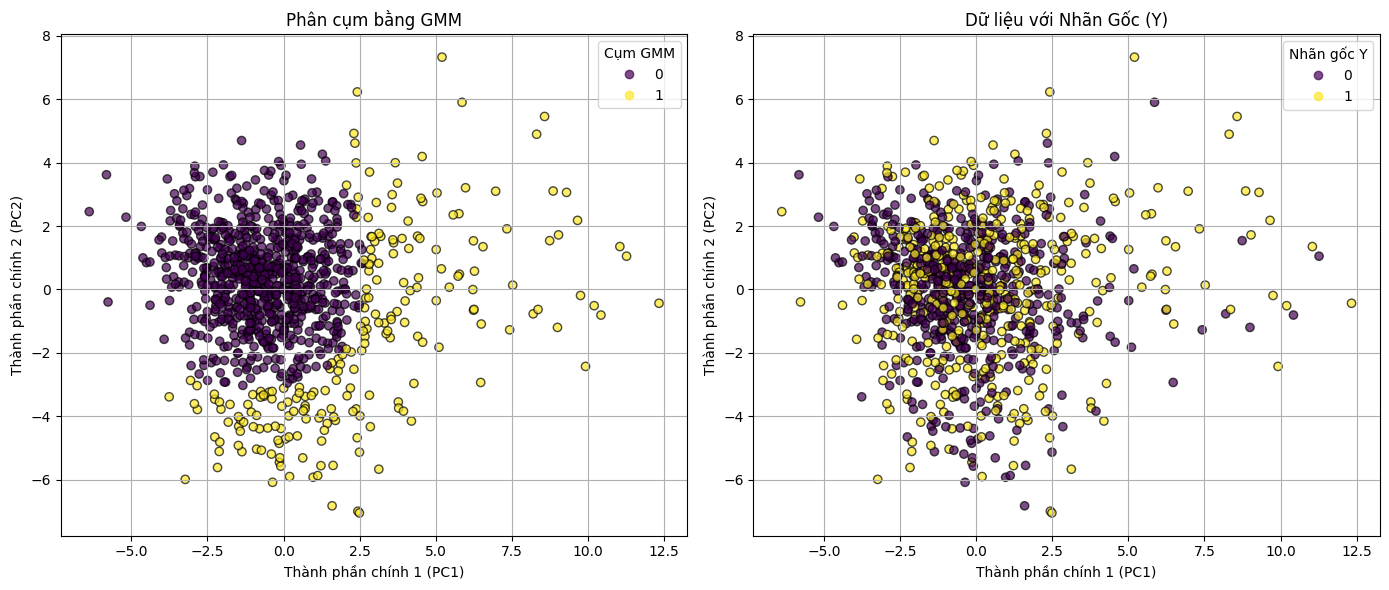
\includegraphics[width=1\linewidth]{img/abideii_plot_gmm.png}
    \caption{Kết quả phân cụm bằng GMM trên bộ dữ liệu ABIDE II}
    \label{fig:abideii_plot_gmm}
\end{figure}

\begin{itemize}
    \item Kết quả phân cụm chính xác \textbf{56.7\%} sau khi nối nhãn với cụm phù hợp (bằng thuật toán Hungary). \texttt{Accuracy:} \texttt{0.567}. \texttt{Recall:} \texttt{0.266}. \texttt{Precision:} \texttt{0.564}.  \texttt{F1-score:} \texttt{0.361}. 
\end{itemize}

\subsection{Nhận xét kết quả phân cụm}
\paragraph{}{Khi áp dụng cả hai thuật toán K-Means và GMM lên bộ dữ liệu ABIDE II (sau khi giảm chiều bằng PCA xuống còn 2 thành phần chính), chúng ta có thể đưa ra một số nhận xét sau:}

\begin{itemize}
    \item Với giá trị F1-score khá thấp nên cả hai thuật toán K-Means và GMM đều cho thấy hiệu suất phân cụm chưa cao khi đánh giá dựa trên nhãn thực tế, với độ chính xác (Accuracy) chỉ nhỉnh hơn một chút so với mức ngẫu nhiên. Điều này cho thấy rằng cấu trúc tự nhiên của dữ liệu không dễ dàng tách thành hai cụm tương ứng hoàn toàn với hai nhóm Cancel và Normal.
    \item Đặc biệt, chỉ số Recall ở cả hai thuật toán đều khá thấp, cho thấy mô hình gặp khó khăn trong việc xác định đúng các trường hợp thuộc nhóm "Cancer" (nếu giả định "Cancer" là lớp positive). Precision tuy cao hơn Recall nhưng vẫn ở mức trung bình.
    \item Quan sát biểu đồ trực quan (Hình 5 và Hình 6), cả K-Means và GMM đều cho thấy sự chồng lấn đáng kể giữa các cụm dữ liệu. Không có một ranh giới rõ ràng nào có thể tách biệt hoàn toàn hai nhóm bệnh nhân. Điều này lý giải tại sao độ chính xác đạt được không cao. Mặc dù có ghi nhận rằng nhãn "Normal" có mật độ cao hơn ở trung tâm, sự phân bố tổng thể vẫn rất phức tạp.
\end{itemize}

\pagebreak